\section{质点的角动量定理和角动量守恒定律}
\subsection{基本概念}
定义：质点对某一给定点$O$的位矢$\vec{r}$与质点动量$\vec{p}$的矢积为质点对给定点的角动量。
$$\vec{L}=\vec{r}\times \vec{p}$$

大小：$L=pr\sin{\varphi}$

方向：垂直于位矢$\vec{r}$和动量$\vec{p}$所组成的平面。指向$\vec{r}$经小于$180^{\circ}$的角转到$\vec{p}$的右手螺旋前进的方向。
	\begin{figure}[h]
	\centering
	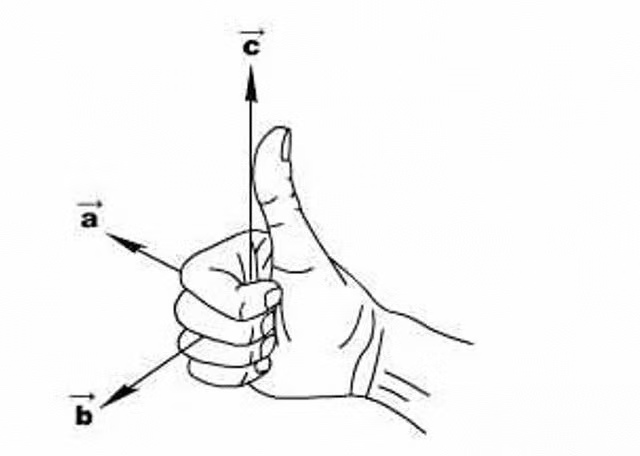
\includegraphics[width=0.5\textwidth]{images/cross.jpg}
	\caption{叉乘的右手定则}
   \end{figure}

单位：$kg\cdot m^2/s$

标矢性：矢量

意义：描述物体的转动特征。

\subsection{引起变化的因素}
\subsubsection{质点的角动量定理}
内容：质点对给定点的角动量随时间的变化率等于作用于质点的合力对该点的力矩。

推导：$$\frac{\mathbf{d}\vec{L}}{\mathbf{d}t}=\frac{\mathbf{d}(\vec{r}\times\vec{p})}{\mathbf{d}t}=\frac{\mathbf{d}\vec{r}}{\mathbf{d}t}\times\vec{p}+\vec{r}\times\frac{\mathbf{d}\vec{p}}{\mathbf{d}t}=\vec{r}\times\frac{\mathbf{d}\vec{p}}{\mathbf{d}t}=\vec{r}\times\vec{F}$$

注意：使用定理时，力矩中的位矢$\vec{r}$和角动量中的位矢$\vec{r}$应相对同一给定点$O$。

\subsubsection{力矩}
定义：力的作用点相对给定点的位矢$\vec{r}$与力$\vec{F}$的矢积为力对给定点的力矩。

单位：$N\cdot m$（牛顿米）

标矢性：矢量

[辨别]力矩与功：$\sin\varphi\text{与}\cos\varphi$、$\vec{r}$与$\mathbf{d}\vec{r}$、矢量与标量

\subsection{质点的角动量守恒定律}
内容：如果作用在质点上的合力对某给定点$O$的力矩为零，则质点对该点的角动量在运动过程中保持不变。

经典场景：质点在有心力作用下运动，角动量守恒。

[例]圆周运动、行星在公转轨道上运动……

\subsection{推广：质点系}
\subsubsection{质点系的角动量定理}
内容：质点系对给定点的角动量随时间的变化率等于外力对该点力矩的矢量和。将$\sum\vec{M_{i\text{外}}}$简写为$\vec{M}$，得
$$\vec{M}=\frac{\mathbf{d}\vec{L}}{\mathbf{d}t}$$

外力与内力：由牛顿第三定律可知，成对出现的内力对给定点的力矩矢量和为零
（类似于冲量，区别于功）。

\subsubsection{质点系的角动量守恒定律}
内容：如果$M=0$，得
$$\vec{L}=\text{常矢量}$$

